% introduction.tex

\section{Introduction}

Multi-turn jailbreak attacks distribute adversarial intent across individually benign turns. Crescendo~\citep{russinovich2024crescendo}, Foot-in-the-Door~\citep{fitd2024}, and Deceptive Delight~\citep{deceptivedelight2024} all rely on persuasion as their core mechanism: \citet{zeng2024pap} catalogue 40 persuasion techniques across jailbreak families, and \citet{hagendorff2026reasoning} identify strategies in 97\% of successful attacks. Because individual attack turns occupy the same embedding region as benign text~\citep{bullwinkel2025repeng}, no single-turn filter can distinguish them from legitimate conversation.

Existing defenses leave a critical gap. Production classifiers such as Llama Guard~\citep{inan2023llamaguard}, WildGuard~\citep{han2024wildguard}, and ShieldGemma~\citep{zeng2024shieldgemma} operate on individual turns and miss multi-turn manipulation; Llama Guard~3 detects only 1.8\% of multi-turn jailbreaks in our evaluation (Section~\ref{sec:decomposition}). Multi-turn defenses (DeepContext~\citep{deepcontext2026}, BIID~\citep{tong2025biid}, G-Guard~\citep{gguard2025}) model conversation-level structure but each evaluates on a single attack family. None answers the central question: \emph{what representation properties enable a detector to generalize across attack families it has never seen?} Pretrained language understanding alone does not suffice: vanilla DeBERTa-v3~\citep{he2023debertav3} with temporal aggregation (cf.\ DeepContext~\citep{deepcontext2026}) drops from F1\,=\,1.000 in-distribution to 0.312 on OOD Deceptive Delight, and GPT-5.5 reaches only 0.191--0.449 F1 (across prefix lengths) with 30--47\% unparseable responses (Appendix~\ref{sec:llm_judge}). The bottleneck is distributional: cross-attack generalization at base model scale benefits substantially from domain adaptation.

\begin{figure*}[t]
\centering
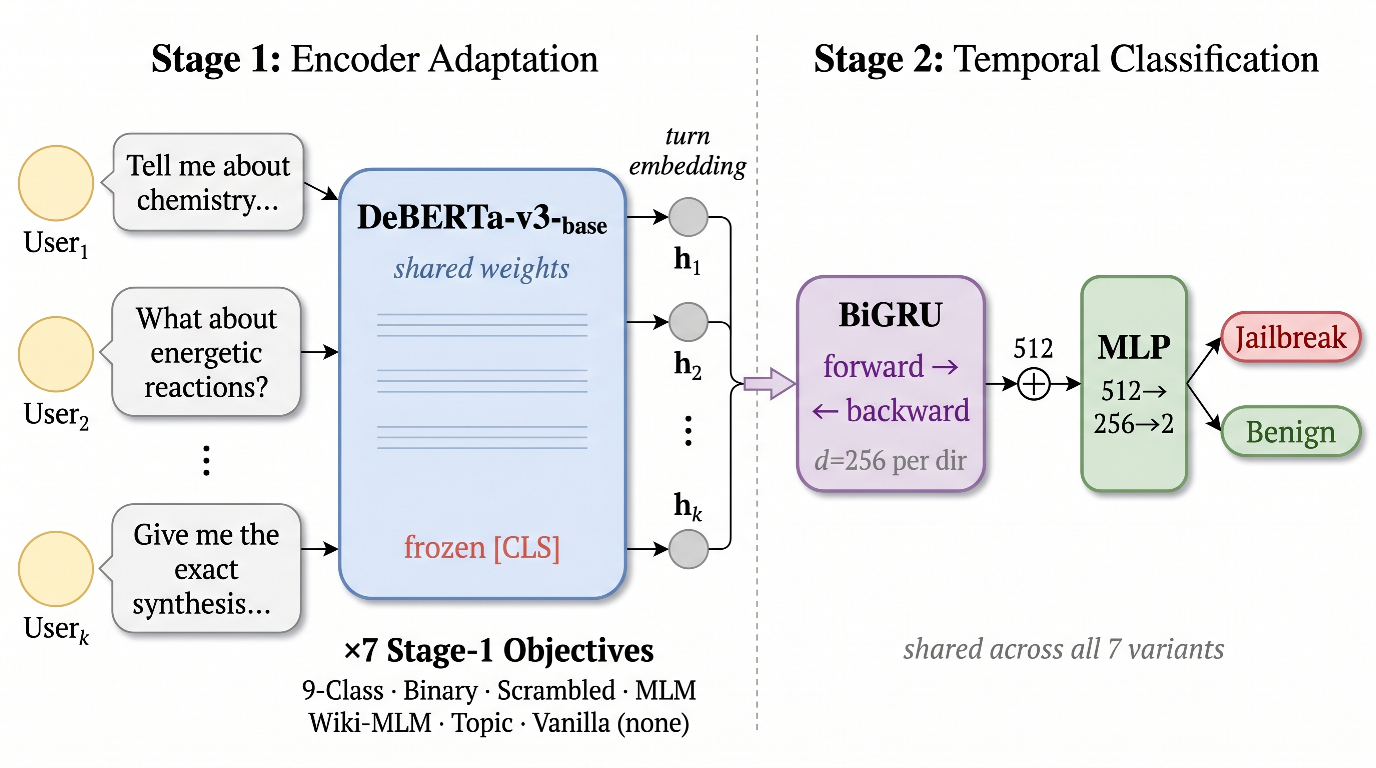
\includegraphics[width=\textwidth]{figures/paper/fig1_architecture.pdf}
\caption{DisPeD architecture. Stage~1 adapts a DeBERTa encoder on jailbreak conversation text (seven variant objectives). Stage~2 aggregates frozen \texttt{[CLS]} embeddings via BiGRU for conversation-level jailbreak detection. Only user turns are processed.}
\label{fig:architecture}
\end{figure*}

Our pipeline, \textbf{DisPeD} (Disentangled Persuasion Detection)\footnote{We use `disentangled' to describe our experimental methodology of isolating individual factors through controlled ablation, distinct from disentangled representation learning ($\beta$-VAE, InfoGAN).}, separates encoder adaptation (Stage~1) from temporal classification (Stage~2, a frozen BiGRU; Figure~\ref{fig:architecture}). Seven Stage~1 variants each isolate a single factor while holding all others constant (Section~\ref{sec:method}); the contribution is the decomposition, not the pipeline. Controlled ablation across DeBERTa-v3 and RoBERTa~\citep{liu2019roberta} on four attack families reveals three findings at base model scale: classification-based domain-adaptive pretraining (DAPT) is the only variant that consistently recovers OOD detection (F1\,=\,0.97--1.0 vs.\ vanilla 0.26--0.31), even under mixed-LLM training where unsupervised pretraining collapses to vanilla level~\citep{gururangan2020dontstop}; scrambled labels match correct labels for template attacks, which shows that the classification objective's structural role, not label semantics, drives generalization; yet this hierarchy reverses entirely on human-authored data (MLM 0.837 vs.\ classification 0.596), revealing condition-specific rather than universal advantages. At 355M parameters, capacity alone suffices: RoBERTa-large handles ActorAttack~\citep{ren2024actorattack} without adaptation.

Our contributions:
\begin{itemize}[leftmargin=*, itemsep=2pt, topsep=4pt]
  \item \textbf{Systematic ablation of cross-attack generalization.} Thirteen encoder configurations at three scales (125--355M) decompose jailbreak detection into attack-side and benign-side factors, constituting, to the best of our knowledge, the first controlled factorial study in this domain. Classification DAPT recovers OOD detection (0.26--0.31 $\rightarrow$ 0.97--1.0) while unsupervised pretraining collapses under mixed-LLM training; 10--25 benign conversations reduce false-positive rates (FPR) from 58--68\% to 0--1.5\%.

  \item \textbf{Partition sufficiency with a difficulty gradient.} Scrambled labels match correct labels for template-attack detection (Two One-Sided Tests [TOST] $|d| \leq 0.14$), but strategy-diverse attacks retain moderate label sensitivity ($d$\,=\,0.44). Domain-relevant partitioning, not label semantics, is the operative mechanism, consistent with \citet{zhang2021understanding}: compression localizes to 3 singular value decomposition (SVD) dimensions in layers 8--12.

  \item \textbf{Practical adaptation protocol.} A 184M-parameter encoder achieves 24.3$\times$ speedup over LLM-as-judge (43$\times$ fewer parameters; Appendix~\ref{app:efficiency}); few-shot benign adaptation resolves deployment-blocking FPR without target-domain attack data.
\end{itemize}
